\documentclass[a4paper,11pt]{article}

\usepackage[utf8]{inputenc}
\usepackage[top=2cm, left = 2cm , right=2cm , bottom=2cm]{geometry}
\usepackage{amsmath}
\usepackage{graphicx}
\usepackage{float}
\usepackage{listings}
\usepackage[brazil]{babel}
\usepackage{multicol}

\usepackage{color}

\definecolor{mygreen}{rgb}{0,0.6,0}
\definecolor{mygray}{rgb}{0.5,0.5,0.5}
\definecolor{mymauve}{rgb}{0.58,0,0.82}

\lstset{
  backgroundcolor=\color{white},   % choose the background color; you must add
                                   % \usepackage{color} or \usepackage{xcolor};
                                   % should come as last argument
  basicstyle=\footnotesize\sffamily,  % the size of the fonts
  breakatwhitespace=false,         % sets if automatic breaks should only happen
                                   % at whitespace
  breaklines=true,                 % sets automatic line breaking
  captionpos=b,                    % sets the caption-position to bottom
  commentstyle=\color{mygreen},    % comment style
  escapeinside={\%*}{*)},          % if you want to add LaTeX within your code
  extendedchars=true,              % lets you use non-ASCII characters; for
                                   % 8-bits encodings only, does not work with
                                   % UTF-8
  frame=single,	                 % adds a frame around the code
  keepspaces=true,                 % keeps spaces in text, useful for keeping
                                   % indentation of code (possibly needs
                                   % columns=flexible)
  keywordstyle=\color{blue},       % keyword style
  language=Matlab,                 % the language of the code
  numbers=left,                    % where to put the line-numbers; possible
                                   % values are (none, left, right)
  numbersep=5pt,                   % how far the line-numbers are from the code
  numberstyle=\tiny\color{mygray}, % the style that is used for the line-numbers
  rulecolor=\color{black},         % if not set, the frame-color may be changed
                                   % on line-breaks within not-black text
                                   % (e.g. comments (green here))
  showspaces=false,                % show spaces everywhere adding particular
                                   % underscores; it overrides
                                   % 'showstringspaces'
  showstringspaces=false,          % underline spaces within strings only
  showtabs=false,                  % show tabs within strings adding particular
                                   % underscores
  stepnumber=2,                    % the step between two line-numbers. If it's
                                   % 1, each line will be numbered
  stringstyle=\color{mymauve},     % string literal style
  tabsize=2,                       % sets default tabsize to 2 spaces
  title=\lstname                   % show the filename of files included with
                                   % \lstinputlisting; also try caption instead
                                   % of title
}

\pagestyle{plain}

\graphicspath{{./Imagens/}}

\begin{document}	

\begin{center}
\textbf{Pré-relatório Experiência 5} \\
\hspace{5pt}
Prof. Marconi Kolm Madrid \\
EA722 - 2017/2
\end{center}

\begin{center}
Danilo Pereira Titato - RA 122541 \\
Giovani Granzotto Oliani - RA 146253 \\
Pedro Gabriel Calixto Mendonça - RA 118363
\end{center}

\textbf{1.}

Função de transferência $X_1\left(s\right) / R\left(s\right)$:

\begin{gather*}
    X_1\left(s\right) = \frac{N_1\left(s\right)}{D\left(s\right)} \cdot k_{hw}
        \cdot G_c\left(s\right) \cdot \left(R\left(s\right) -
        X_1\left(s\right)\right) \\
    X_1\left(s\right) \cdot \left(1 + k_{hw} \cdot
        \frac{N_1\left(s\right)}{D\left(s\right)} \cdot G_c\left(s\right)\right)
        = k_{hw} \cdot \frac{N_1\left(s\right)}{D\left(s\right)} \cdot
        G_c\left(s\right) \cdot R\left(s\right) \\
    \frac{X_1\left(s\right)}{R\left(s\right)} = \frac{k_{hw} \cdot
        \frac{N_1\left(s\right)}{D\left(s\right)} \cdot G_c\left(s\right)}
        {1 + k_{hw} \cdot \frac{N_1\left(s\right)}{D\left(s\right)} \cdot
        G_c\left(s\right)} \\ \\
    X_2\left(s\right) = \frac{N_2\left(s\right)}{N_1\left(s\right)} \cdot
        X_1\left(s\right) =
        \frac{N_2\left(s\right)}{N_1\left(s\right)} \cdot \frac{k_{hw} \cdot
        \frac{N_1\left(s\right)}{D\left(s\right)} \cdot G_c\left(s\right)}{1 +
        k_{hw} \cdot \frac{N_1\left(s\right)}{D\left(s\right)} \cdot
        G_c\left(s\right)} =
        \frac{k_{hw} \cdot \frac{N_2\left(s\right)}{D\left(s\right)} \cdot
        G_c\left(s\right)}{1 + k_{hw} \cdot \frac{N_1\left(s\right)}
        {D\left(s\right)} \cdot G_c\left(s\right)}
\end{gather*}

Para o controlador $PD_1$ ($k_p = 1.0, k_d = 0.03$), tem-se os seguintes pólos e
zeros:

\begin{figure}[H]
\centering
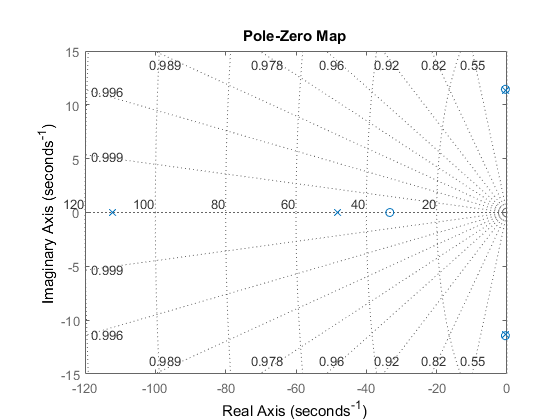
\includegraphics{q01-pd1x1-pzmap}
\caption{Pólos e zeros de $X_1\left(s\right)$ para $PD_1$}
\end{figure}

\begin{figure}[H]
\centering
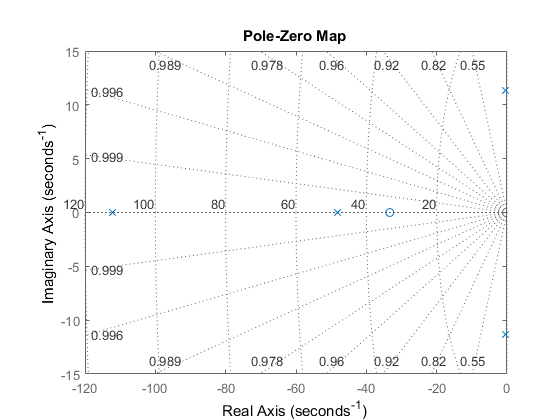
\includegraphics{q01-pd1x2-pzmap}
\caption{Pólos e zeros de $X_2\left(s\right)$ para $PD_1$}
\end{figure}

$X_1\left(s\right)$:

\begin{multicols}{2}
    Pólos (rad/s):
    \begin{itemize}
        \item -112.14
        \item -48.28
        \item -0.50 + 11.32i
        \item -0.50 - 11.32i
    \end{itemize}
\columnbreak
    Zeros (rad/s):
    \begin{itemize}
        \item -33.3333
        \item -0.4570 + 11.4425i
        \item -0.4570 - 11.4425i
    \end{itemize}
\end{multicols}

$X_2\left(s\right)$:

\begin{multicols}{2}
    Pólos (rad/s):
    \begin{itemize}
        \item -112.14
        \item -48.28
        \item -0.50 + 11.32i
        \item -0.50 - 11.32i
    \end{itemize}
\columnbreak
    Zeros (rad/s):
    \begin{itemize}
        \item -33.3333
    \end{itemize}
\end{multicols}

Pode-se ver que os pólos são os mesmos para $X_1\left(s\right)$ e
$X_2\left(s\right)$. Existe também um zero em comum. A diferença dos zeros é a
presença de um par de zeros contido no plano imaginário em $X_1\left(s\right)$.

Pólo(s) dominante(s) de $PD_1$:

\begin{multicols}{2}
    $X_1\left(s\right) / R\left(s\right)$:
    \begin{itemize}
        \item $-0.50 \pm 11.32i$
    \end{itemize}
\columnbreak
    $X_2\left(s\right) / R\left(s\right)$:
    \begin{itemize}
        \item $-0.50 \pm 11.32i$
    \end{itemize}
\end{multicols}

\pagebreak

Já para o controlador $PD_2$ ($k_p = 0.05, k_d = 0.01$), tem-se os seguintes
pólos e zeros:

\begin{figure}[H]
\centering
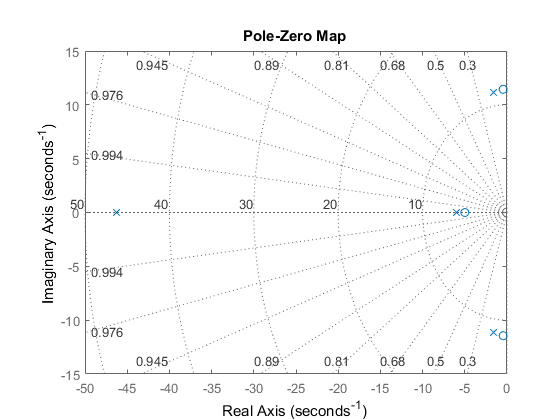
\includegraphics{q01-pd2x1-pzmap}
\caption{Pólos e zeros de $X_1\left(s\right)$ para $PD_2$}
\end{figure}

\begin{figure}[H]
\centering
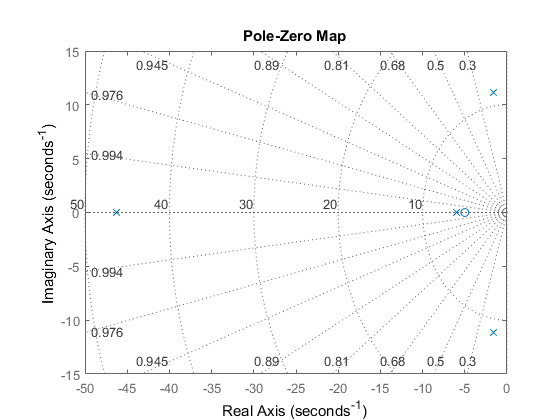
\includegraphics{q01-pd2x2-pzmap}
\caption{Pólos e zeros de $X_2\left(s\right)$ para $PD_2$}
\end{figure}

$X_1\left(s\right)$:

\begin{multicols}{2}
    Pólos (rad/s):
    \begin{itemize}
        \item -46.2243
        \item -5.9304
        \item -1.6007 + 11.1483i
        \item -1.6007 - 11.1483i
    \end{itemize}
\columnbreak
    Zeros (rad/s):
    \begin{itemize}
        \item -5.0000
        \item -0.4570 + 11.4425i
        \item -0.4570 - 11.4425i
    \end{itemize}
\end{multicols}

$X_2\left(s\right)$:

\begin{multicols}{2}
    Pólos (rad/s):
    \begin{itemize}
        \item -46.2243
        \item -5.9304
        \item -1.6007 + 11.1483i
        \item -1.6007 - 11.1483i
    \end{itemize}
\columnbreak
    Zeros (rad/s):
    \begin{itemize}
        \item -5.0000
    \end{itemize}
\end{multicols}

Pode-se ver que os pólos são os mesmos para $X_1\left(s\right)$ e
$X_2\left(s\right)$. Existe também um zero em comum. A diferença dos zeros é a
presença de um par de zeros contido no plano imaginário em $X_1\left(s\right)$.

Pólo(s) dominante(s) de $PD_2$:

\begin{multicols}{2}
    $X_1\left(s\right) / R\left(s\right)$:
    \begin{itemize}
        \item $-1.6007 \pm 11.1483i$
    \end{itemize}
\columnbreak
    $X_2\left(s\right) / R\left(s\right)$:
    \begin{itemize}
        \item $-1.6007 \pm 11.1483i$
    \end{itemize}
\end{multicols}

Pode-se perceber que os pólos dominantes são os mesmos em $X_1\left(s\right)$ e
$X_2\left(s\right)$, tanto para o controlador $PD_1$ quanto para $PD_2$.

\pagebreak

As respostas temporais da entrada ao degrau de $X_1\left(s\right)$ e
$X_2\left(s\right)$, para os controladores $PD_1$ e $PD_2$, são:

\begin{figure}[H]
\centering
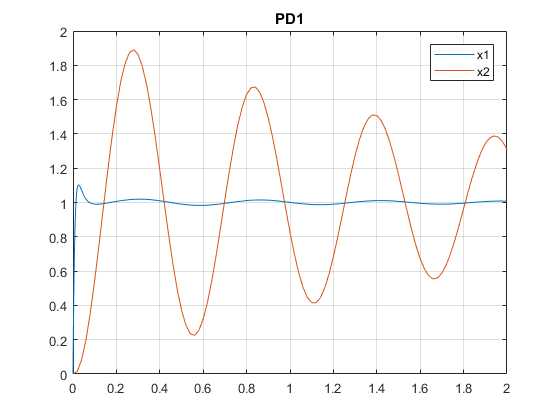
\includegraphics[scale=0.9]{q01-pd1-step}
\caption{Respostas ao degrau usando $PD_1$}
\end{figure}

\begin{figure}[H]
\centering
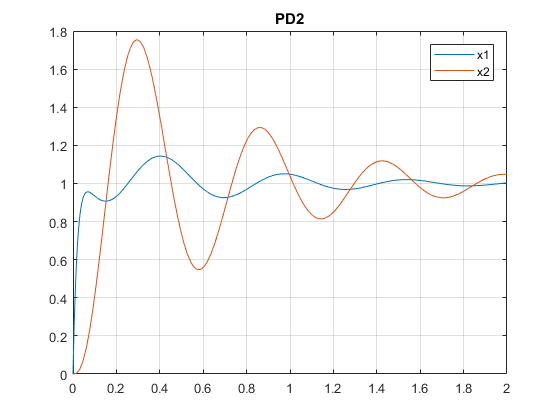
\includegraphics[scale=0.9]{q01-pd2-step}
\caption{Respostas ao degrau usando $PD_2$}
\end{figure}

Na resposta temporal, vemos que tanto para PD1 como para PD2, o carro oscila
muito. Para o carro 1, porém, percebe-se que há mais oscilação na resposta com
PD2 do que na com PD1. Isso pode ser explicado pela localização dos pólos nas
duas funções de transferência. Com PD1, os pólos dominantes (aqueles conjugados
mais próximos ao eixo imaginário) ficam muito próximos dos zeros, o que anula em
parte o seu forte efeito oscilatório.

Já com PD2, os pólos dominantes ficam um pouco mais à esquerda e distantes dos
zeros. Por conta disso, o seu efeito oscilatório é menos atenuado pelos pólos,
o que resulta em uma resposta temporal com mais oscilação. \\

\textbf{2.}

Diagrama de Bode da função de transferência de malha aberta
$k_{hw} G_c\left(s\right) \cdot \frac{N_1\left(s\right)}{D\left(s\right)}$:

\begin{figure}[H]
\centering
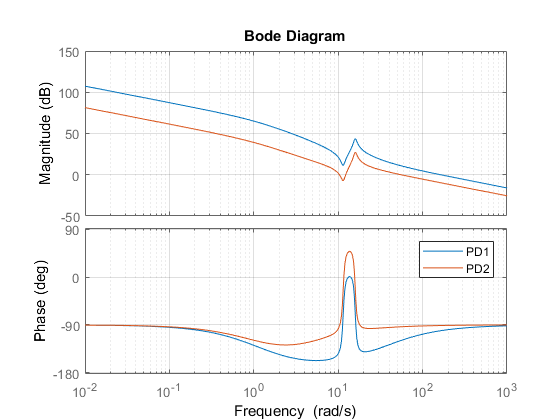
\includegraphics{q02-aberta}
\caption{Diagram de Bode em malha aberta}
\end{figure}

A função de transferência de Bode para a malha fechada
$\frac{X_1\left(s\right)}{F_d\left(s\right)}$ é:

\begin{gather*}
    X_1\left(s\right) = \frac{N_1\left(s\right)}{D\left(s\right)} \cdot
        \left\{F_d\left(s\right) + \left[k_{hw} \cdot G_c\left(s\right) \cdot
        \left(- X_1\left(s\right)\right)\right]\right\} \implies \\
    X_1\left(s\right) \cdot \left(1 + \frac{N_1\left(s\right)}{D\left(s\right)}
        \cdot G_c\left(s\right)\right) =
        \frac{N_1\left(s\right)}{D\left(s\right)} \cdot F_d\left(s\right)
        \implies \\
    \frac{X_1\left(s\right)}{F_d\left(s\right)} =
        \frac{\frac{N_1\left(s\right)}{D\left(s\right)}}{1 +
        \frac{N_1\left(s\right)}{D\left(s\right)} \cdot G_c\left(s\right)}
\end{gather*}

\pagebreak

Diagrama de Bode da função de transferência de malha fechada
$\frac{X_1\left(s\right)}{F_d\left(s\right)}$:

\begin{figure}[H]
\centering
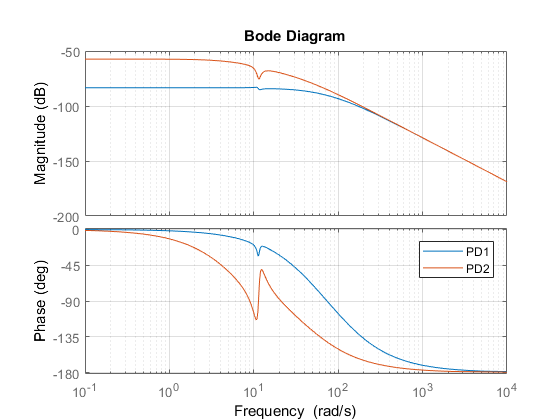
\includegraphics{q02-fechada}
\caption{Diagram de Bode em malha fechada}
\end{figure}

\textbf{3.}
Para altas frequências, PD1 e PD2 se igualam assintoticamente, tanto para a
malha aberta quanto para a malha fechada. 

Já para as altas frequências, PD1 tem maior magnitude que PD2 para a malha
aberta, enquanto para a malha fechada PD1 possui menor magnitude que PD2. Entre
a malha aberta e a malha fechada, PD1 tem sua magnitude reduzida a ponto de ser
menor que PD2, mostrando, então, que PD1 atenua mais os distúrbios do que PD2. 

\end{document}